\chapter{Testing}\label{ch-09}

\lecturemeta{Capitolo originale: 9 --- Testing \quad\textbullet\quad Antonio Brogi}{Appunti di Emiliano Sescu (github.com/Faxatos), cap. 9}

\begin{boxdefinition}{Testing}

Il \textbf{testing} è il processo sistematico con cui si esegue un
programma usando dati che simulano l'input dell'utente, per verificare
che il software funzioni come previsto e rispetti i requisiti.

\end{boxdefinition}

Il testing serve a osservare in modo metodico il comportamento del
programma. Il principio di base è \textbf{confrontare il comportamento
atteso con quello reale} durante l'esecuzione:

\begin{itemize}
\tightlist
\item
  se il comportamento osservato è quello atteso, il test \textbf{passa};
\item
  se si discosta da quello atteso, il test \textbf{fallisce}.
\end{itemize}

Alcuni tipi di test:

\begin{itemize}
\tightlist
\item
  \textbf{Test funzionale} (\emph{functional testing}): verifica che
  l'applicazione svolga le sue funzioni come previsto. Si valutano le
  singole feature per controllare che rispettino i requisiti, guardando
  input, output e comportamento del sistema in varie condizioni.
\item
  \textbf{Test con gli utenti} (\emph{user testing}, o test di
  usabilità): valuta il software dal punto di vista dell'utente finale,
  per verificare che sia facile e intuitivo da usare e che risponda ai
  bisogni di chi lo userà. Spesso coinvolge utenti reali, per trovare
  problemi di usabilità, difetti di design o punti da migliorare.
\item
  \textbf{Test di prestazioni e di carico} (\emph{performance and load
  testing}): il test di prestazioni misura reattività, velocità ed
  efficienza in condizioni diverse. Il test di carico, un suo
  sottoinsieme, valuta come si comporta il sistema con livelli simulati
  o previsti di utenti contemporanei. Aiutano a trovare colli di
  bottiglia, misurare la scalabilità e assicurare buone prestazioni con
  carichi diversi.
\item
  \textbf{Test di sicurezza} (\emph{security testing}): cerca
  vulnerabilità e punti deboli per proteggere il sistema da minacce e
  accessi non autorizzati. Valuta la resistenza ad attacchi, furti di
  dati e manipolazioni, e aiuta a garantire che i dati sensibili siano
  protetti e che si rispettino gli standard di sicurezza.
\end{itemize}

\begin{boxwarning}{Il limite del testing}

Il testing può mostrare la \textbf{presenza} di bug, ma \textbf{mai la
loro assenza} (Dijkstra): non sostituisce la verifica formale del
software.

\end{boxwarning}

Il resto del capitolo approfondisce il test funzionale e il test di
sicurezza.

\section{Test funzionale}\label{test-funzionale}

Il \textbf{test funzionale} è un insieme completo di test che
garantiscono che \textbf{tutto il codice venga eseguito almeno una
volta}, per verificare il comportamento complessivo del sistema. Il
testing deve iniziare \textbf{dal giorno in cui si comincia a scrivere
codice}, e i test automatici semplificano il ciclo sviluppo-test.

Il test funzionale è un'attività \textbf{a fasi}: il processo è
organizzato in fasi distinte (Fig. 9.1). Le fasi non sono rigidamente in
sequenza e spesso si sovrappongono. Inoltre il \textbf{test di
regressione} si fa continuamente, in ogni fase, per controllare che
modifiche o nuove feature non introducano difetti in funzionalità già
testate. Dividere il lavoro in fasi aiuta a trovare e risolvere i
problemi ai diversi livelli dello sviluppo.

\begin{figure}[H]
\centering
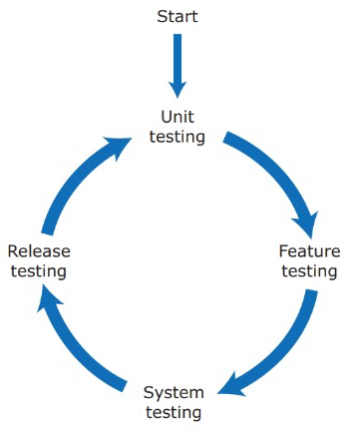
\includegraphics[width=0.37\linewidth,height=0.45\textheight,keepaspectratio]{images/09-testing_fig9-1_ciclo-functional-testing.png}
\caption{Il ciclo di vita del test funzionale.}
\end{figure}

\subsection{Unit testing}\label{unit-testing}

L'obiettivo dello \textbf{unit testing} è testare le \textbf{unità del
programma} (es. funzioni, metodi) \textbf{in isolamento}.

\begin{boxdefinition}{Principio dello unit test}

Se un'unità di programma si comporta come previsto per un insieme di
input che hanno alcune caratteristiche in comune, si comporterà allo
stesso modo per un insieme più grande di input con le stesse
caratteristiche.

\end{boxdefinition}

\begin{boxexample}{Esempio}

Se un programma si comporta correttamente con gli input 1, 5, 17, 45,
99, si può concludere che elaborerà correttamente anche tutti gli altri
interi tra 1 e 99.

\end{boxexample}

Per questo è importante individuare le \textbf{partizioni di
equivalenza}: insiemi di input che vengono trattati allo stesso modo da
un pezzo di codice. Poi si testa il programma con diversi input presi da
ogni partizione. I programmatori sbagliano spesso proprio sui
\textbf{limiti} delle partizioni, quindi conviene usare i valori di
confine come input.

Linee guida per gli unit test:

\begin{itemize}
\tightlist
\item
  \textbf{Testa i casi limite}: se la partizione ha un limite inferiore
  e superiore (lunghezza delle stringhe, numeri, \ldots), scegli input
  ai bordi dell'intervallo.
\item
  \textbf{Forza gli errori}: scegli input che facciano generare al
  sistema tutti i messaggi di errore, e input che dovrebbero produrre
  output non validi.
\item
  \textbf{Riempi i buffer}: scegli input che facciano traboccare tutti i
  buffer di input.
\item
  \textbf{Ripeti}: ripeti più volte lo stesso input o la stessa serie di
  input.
\item
  \textbf{Overflow e underflow}: se il programma fa calcoli numerici,
  scegli input che producano numeri molto grandi o molto piccoli.
\item
  \textbf{Non dimenticare null e zero}: se il programma usa puntatori o
  stringhe, testa sempre con puntatori e stringhe nulli; con le
  sequenze, testa la sequenza vuota; con i numeri, testa sempre lo zero.
\item
  \textbf{Tieni il conto}: con liste e trasformazioni di liste, conta
  gli elementi di ogni lista e controlla che i conti tornino dopo ogni
  trasformazione.
\item
  \textbf{Uno è diverso}: se il programma lavora su sequenze, testa
  sempre anche sequenze con un solo elemento.
\end{itemize}

\begin{boxexample}{Partizioni e limiti in pratica}

Una funzione accetta un'età tra 18 e 65. Le partizioni sono: minore di
18 (non valida), 18-65 (valida), maggiore di 65 (non valida). Oltre a un
valore ``normale'' per ogni partizione (es. 10, 40, 80), si testano i
confini: 17, 18, 65, 66.

\end{boxexample}

\subsection{Feature testing}\label{feature-testing}

Una feature implementa una funzionalità utile per l'utente. L'obiettivo
del \textbf{feature testing} è verificare che quella funzionalità sia
implementata come previsto e risponda ai bisogni reali degli utenti. Le
feature di solito sono realizzate da più unità che interagiscono, quindi
ci sono due tipi di test:

\begin{itemize}
\tightlist
\item
  \textbf{Test di interazione}: verificano le interazioni tra unità (di
  solito scritte da sviluppatori diversi). Possono anche scoprire bug
  nelle singole unità sfuggiti agli unit test.
\item
  \textbf{Test di utilità} (\emph{usefulness tests}): verificano che la
  feature faccia quello che gli utenti probabilmente vogliono. Il
  \textbf{Product Manager} dovrebbe partecipare alla loro progettazione.
\end{itemize}

I test delle feature si ricavano da \textbf{scenari} o \textbf{user
story}.

\begin{boxexample}{Da user story a test}

\textbf{User story} --- Registrazione: ``Come utente, voglio poter
accedere senza creare un nuovo account, così non devo ricordare un altro
login e un'altra password.''

\textbf{Test} --- Schermata di login iniziale:

\begin{itemize}
\tightlist
\item
  verificare che, quando l'utente clicca su ``Accedi con Google'', venga
  mostrata correttamente la schermata che chiede le credenziali Google;
\item
  verificare che il login vada a buon fine se l'utente ha già fatto
  l'accesso a Google.
\end{itemize}

\end{boxexample}

\subsection{System testing}\label{system-testing}

L'obiettivo del \textbf{system testing} è testare il sistema \textbf{nel
suo insieme}, per:

\begin{itemize}
\tightlist
\item
  scoprire interazioni inattese o indesiderate tra le feature;
\item
  capire se le feature lavorano bene insieme per supportare ciò che gli
  utenti vogliono davvero fare;
\item
  assicurarsi che il sistema funzioni come previsto nei diversi ambienti
  in cui verrà usato;
\item
  testare reattività, throughput, sicurezza e gli altri attributi di
  qualità.
\end{itemize}

Un consiglio per creare i test di sistema è usare scenari e user story
per individuare i \textbf{percorsi completi} (\emph{end-to-end}) degli
utenti, perché si vuole testare il flusso dei dati attraverso moduli
diversi.

\subsection{Release testing}\label{release-testing}

Il \textbf{release testing} testa un sistema pronto per essere
rilasciato ai clienti, nel suo \textbf{ambiente operativo reale} (non in
un ambiente di test). L'obiettivo è \textbf{decidere se il sistema è
abbastanza buono da essere rilasciato}, non trovare bug.

Serve perché preparare un sistema per il rilascio vuol dire
impacchettarlo per il deploy, installare software e librerie necessari e
configurare i parametri, e in questi passaggi si possono fare errori. Se
il software è nel cloud, si può usare un processo di \textbf{rilascio
continuo} automatico.

\section{Test di sicurezza}\label{test-di-sicurezza}

Gli obiettivi del \textbf{test di sicurezza} sono:

\begin{itemize}
\tightlist
\item
  trovare le \textbf{vulnerabilità} che un attaccante potrebbe
  sfruttare;
\item
  fornire prove convincenti che il sistema è \textbf{abbastanza sicuro}.
\end{itemize}

Trovare vulnerabilità è più difficile che trovare bug, perché bisogna
testare qualcosa che il software \textbf{NON} deve fare (potenzialmente
infiniti test). I normali test funzionali possono non rivelare le
vulnerabilità, e anche il software su cui si appoggia il prodotto
(sistema operativo, librerie, database, \ldots) può contenerne.

Un test di sicurezza completo richiede conoscenze specialistiche (es.
coinvolgere esperti esterni per il \textbf{penetration testing}, che
costa molto). Di solito le aziende usano un \textbf{approccio basato sul
rischio}: individuano i principali rischi di sicurezza del prodotto e
scrivono test che dimostrino che il prodotto se ne protegge. Alcuni test
si possono automatizzare, altri richiedono per forza controlli manuali
del comportamento e dei file.

Esempi di rischi di sicurezza:

\begin{itemize}
\tightlist
\item
  un attaccante non autorizzato entra nel sistema usando credenziali
  autorizzate;
\item
  una persona autorizzata accede a risorse che le sono vietate;
\item
  il sistema di autenticazione non riconosce un attaccante non
  autorizzato;
\item
  un attaccante accede al database con una SQL injection;
\item
  gestione scorretta delle sessioni HTTP;
\item
  i cookie di sessione HTTP finiscono in mano a un attaccante;
\item
  dati riservati non cifrati;
\item
  chiavi di cifratura finite in mano a un potenziale attaccante.
\end{itemize}

\begin{boxtip}{Pensa come un attaccante}

Quando si testa la sicurezza bisogna ragionare come un
\textbf{attaccante}, non come un utente normale: provare apposta a fare
le cose sbagliate e ripetere le azioni più volte.

\end{boxtip}

\section{Automazione dei test}\label{automazione-dei-test}

I \textbf{test automatici} sono molto usati nelle aziende di prodotto,
perché testare il sistema a mano è noioso e soggetto a errori. I test
eseguibili controllano che il software restituisca il risultato atteso
per certi dati di input (Fig. 9.2).

\begin{boxdefinition}{Struttura di un test automatico (Arrange-Act-Assert)}

\begin{enumerate}
\def\labelenumi{\arabic{enumi}.}
\tightlist
\item
  \textbf{Arrange} (prepara): si prepara il sistema per eseguire il test
  (si definiscono i parametri del test).
\item
  \textbf{Action} (esegui): si chiama l'unità da testare con quei
  parametri.
\item
  \textbf{Assert} (verifica): si dichiara cosa deve essere vero se il
  test va a buon fine.
\end{enumerate}

\end{boxdefinition}

\begin{figure}[H]
\centering
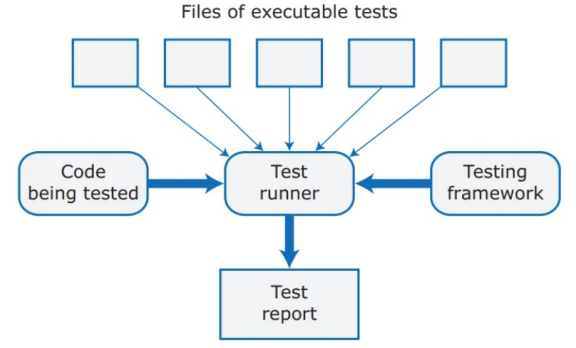
\includegraphics[width=0.63\linewidth,height=0.45\textheight,keepaspectratio]{images/09-testing_fig9-2_test-runner.png}
\caption{Schema del test runner.}
\end{figure}

\begin{boxexample}{Un test con Arrange-Act-Assert (Python)}

\begin{Verbatim}
def test_sconto_10_percento():
    carrello = Carrello(totale=100)        # Arrange
    carrello.applica_sconto(0.10)          # Action
    assert carrello.totale == 90           # Assert
\end{Verbatim}

\end{boxexample}

Esistono framework di test per tutti i linguaggi più usati. Anche il
\textbf{codice dei test può contenere bug}: per ridurre il rischio
conviene scrivere test il più semplici possibile e revisionare i test
insieme al codice che testano.

Gli \textbf{unit test} sono i più facili da automatizzare. Buoni unit
test riducono (ma non eliminano) il bisogno di feature test, ed è un
bene perché i \textbf{test tramite interfaccia grafica} (GUI) sono
costosi da automatizzare (Fig. 9.3): conviene testare tramite le
\textbf{API}. Per controllare che una feature abbia funzionato come
previsto servono più asserzioni.

\begin{figure}[H]
\centering
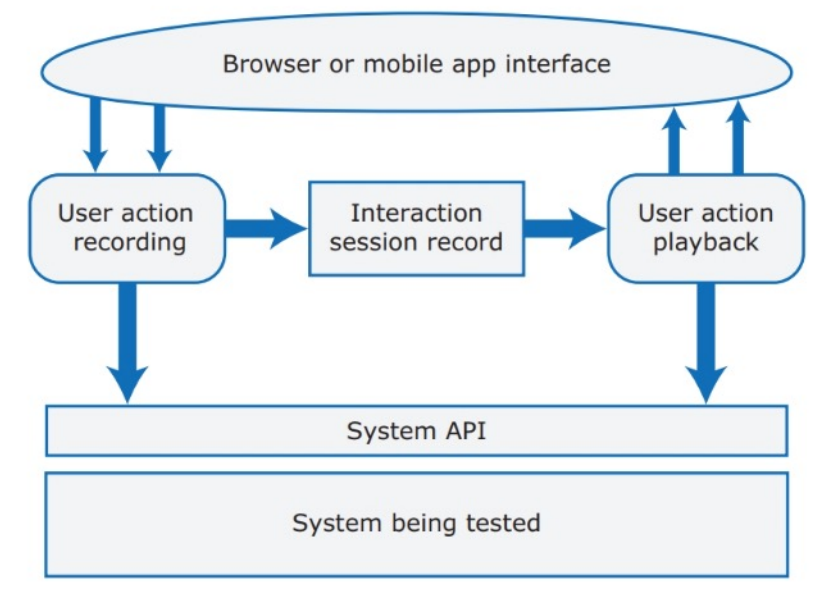
\includegraphics[width=0.65\linewidth,height=0.45\textheight,keepaspectratio]{images/09-testing_fig9-3_test-gui.png}
\caption{Il ciclo del test basato su GUI.}
\end{figure}

\section{Test-Driven Development}\label{test-driven-development}

Alcuni framework Agile, come l'Extreme Programming, sono
\textbf{test-driven}: gli sviluppatori scrivono \textbf{prima i test
eseguibili} e \textbf{poi il codice} che li fa passare. La Fig. 9.4
mostra come il \textbf{Test-Driven Development} (TDD) si inserisce nel
ciclo di sviluppo.

\begin{figure}[H]
\centering
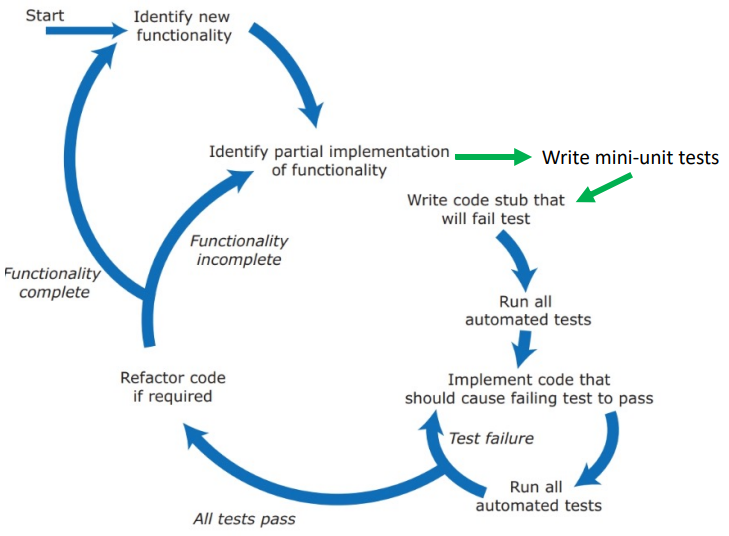
\includegraphics[width=1.00\linewidth,height=0.45\textheight,keepaspectratio]{images/09-testing_fig9-4_tdd.png}
\caption{Il ciclo del Test-Driven Development.}
\end{figure}

\begin{boxtip}{Il ciclo in tre parole: red, green, refactor}

Si scrive un test che fallisce (\textbf{red}), si scrive il codice
minimo per farlo passare (\textbf{green}), si migliora il codice
mantenendo i test verdi (\textbf{refactor}).

\end{boxtip}

Vantaggi:

\begin{itemize}
\tightlist
\item
  \textbf{Approccio sistematico}: i test sono legati chiaramente a parti
  del codice, quindi non ci sono parti non testate.
\item
  I test aiutano a \textbf{capire il codice}.
\item
  \textbf{Debug semplificato} e incrementale.
\item
  \textbf{Codice più semplice} (punto discutibile).
\end{itemize}

Svantaggi:

\begin{itemize}
\tightlist
\item
  è difficile applicare il TDD al \textbf{test di sistema};
\item
  scoraggia i \textbf{cambiamenti radicali} al programma;
\item
  porta a concentrarsi sui test invece che sul problema da risolvere;
\item
  porta a pensare troppo ai dettagli di implementazione invece che alla
  struttura generale del programma;
\item
  è difficile scrivere test con \textbf{``dati sbagliati''}.
\end{itemize}

\section{Code review}\label{code-review}

Il testing ha dei limiti:

\begin{itemize}
\tightlist
\item
  Gli sviluppatori testano il codice in base a \textbf{come hanno
  capito} cosa deve fare. Se hanno capito male, l'errore sarà sia nel
  codice sia nei test.
\item
  I test possono non coprire tutto il codice scritto (il TDD sposta il
  problema sull'incompletezza del codice).
\item
  I test non dicono molto su altre qualità del programma (leggibilità,
  struttura, facilità di evoluzione).
\end{itemize}

Per questo le \textbf{code review} (revisioni del codice) completano il
testing. La Fig. 9.5 mostra come lavora un revisore.

\begin{figure}[H]
\centering
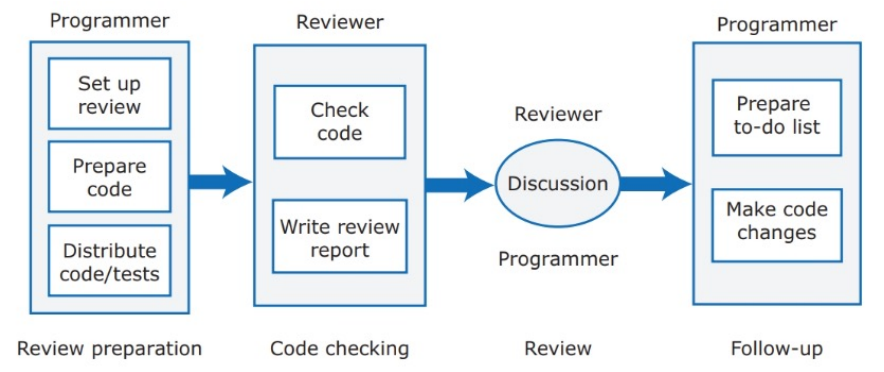
\includegraphics[width=0.80\linewidth,height=0.45\textheight,keepaspectratio]{images/09-testing_fig9-5_code-review.png}
\caption{Il ciclo delle code review.}
\end{figure}

Spesso c'è \textbf{un solo revisore} (dello stesso team DevOps o di un
altro), che può commentare anche la leggibilità e la comprensibilità del
codice. Ogni sessione di review dovrebbe riguardare \textbf{200-400
righe di codice} e può partire in automatico dai commit sui repository
condivisi.

Il revisore usa spesso una \textbf{checklist} con punti generali o
specifici del linguaggio. Esempi:

\begin{itemize}
\tightlist
\item
  (generale) I nomi di variabili e funzioni sono significativi?
\item
  (generale) Sono stati considerati tutti gli errori sui dati, con i
  relativi test?
\item
  (generale) Tutte le eccezioni sono gestite esplicitamente?
\item
  (Python) Si usano parametri di default nelle funzioni?
\item
  (Python) I tipi sono usati in modo coerente?
\item
  (Python) Il livello di indentazione è corretto?
\end{itemize}
